\documentclass[10pt,twocolumn,letterpaper]{article}

\usepackage{dependable_dnn}
\usepackage{times}
\usepackage{epsfig}
\usepackage{graphicx}
\usepackage{amsmath}
\usepackage{amssymb}
\usepackage{subfigure}
\usepackage[table, dvipsnames]{xcolor}

% Include other packages here, before hyperref.

% If you comment hyperref and then uncomment it, you should delete
% egpaper.aux before re-running latex.  (Or just hit 'q' on the first latex
% run, let it finish, and you should be clear).
\usepackage[pagebackref=true,breaklinks=true,letterpaper=true,colorlinks,bookmarks=false]{hyperref}

\iccvfinalcopy % *** Uncomment this line for the final submission

\def\iccvPaperID{} % *** Enter the Paper ID here
\def\httilde{\mbox{\tt\raisebox{-.5ex}{\symbol{126}}}}

% Pages are numbered in submission mode, and unnumbered in camera-ready
\ificcvfinal\pagestyle{empty}\fi

\begin{document}

%%%%%%%%% TITLE - PLEASE UPDATE
\title{End-to-End Object Detection with Transformers\\ {\rm {\normalsize Seungmin Lee (profile2697@gmail.com; 2020-20866), \\Dept. of Electrical and Computer Engineering, Seoul National University}}}   % **** Enter the paper title and student information here

\maketitle
\thispagestyle{empty}

\section{Introduction and Motivation}
Current object detection methods address object detection as a sequential task that predicts object classes after proposing the candidate bounding boxes. Thus, these methods tackle object detection as a combination of a surrogate regression task for boxes proposals and a classification task on the selected proposals. Unfortunately, this kind of approach makes the object detection pipeline complex, requiring a lot of heuristics such as Non-Maximal Suppression~\cite{} or a complicated training scheme~\cite{}.

To address this problem, this paper view object detection as a direct set prediction where the set is a collection of the (class, bounding box coordination) pairs. The changed view simplifies the object detection process by removing the heuristics that encode the human's prior knowledge about object detection.

The authors implement the set predictor using an encoder-decoder transformer and bipartite matching loss. The transformer takes features extracted from a traditional convolutional neural network (CNN) as input tokens and outputs a set of (class, bounding box)s. 

\begin{figure}[b]
	\centering
	\subfigure[The transformer architecture]{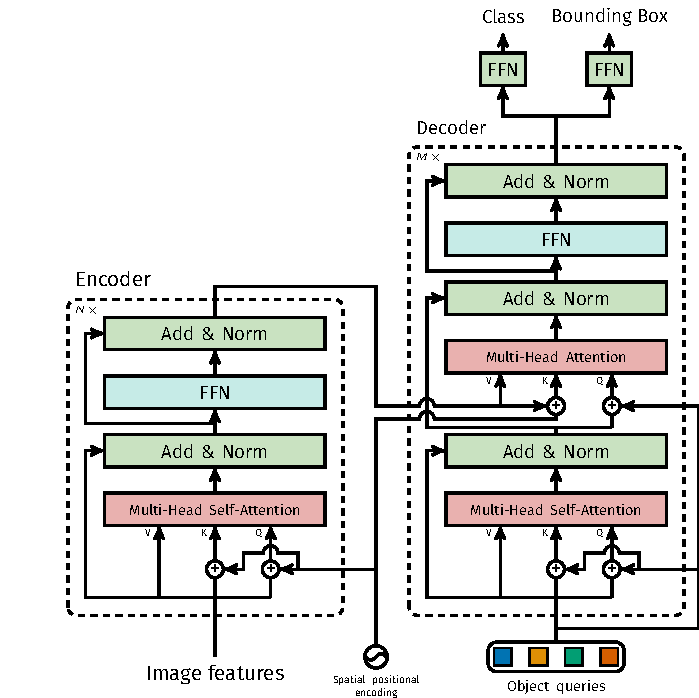
\includegraphics[width=4cm, height=4cm]{assets/transformer.pdf}}
	\subfigure[The encoder resolves instance occlusions]{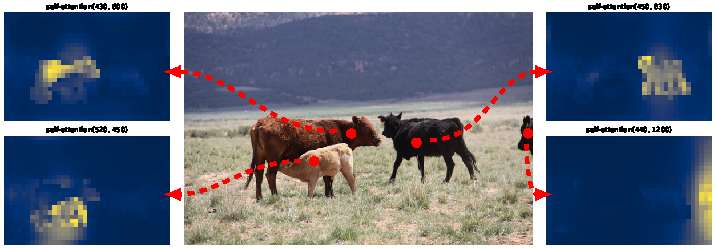
\includegraphics[width=4cm, height=2.5cm]{assets/cows_attn.pdf}}
	\caption{(a) The proposed encoder-decoder transformer architecture, (b) The encoder's attention maps: the encoder separate each instance even though those are occluded.}
	\label{fig:imgs}
\end{figure}

\section{Method}
\subsection{Architecture}
The proposed architecture consists of three main components: a CNN backbone that extracts features used as input tokens for transformer, an encoder-decoder transformer that takes CNN features and transforms the features, and two feed-forward networks that predict classes and bounding box coordinations, respectively. 

The transformer has the typical form as proposed in ~\cite{} except they use additional positional encodings called \textit{object queries} on the decoder. The detailed architecture is shown in Figure~\ref{fig:imgs} (a). 

\subsection{Set Prediction Loss}


\section{Results}

\section{Personal Note}
The main contributions of this paper are two-fold. First, it views object detection as a class-box set prediction rather than a sequential task that classifies object classes in the boxes after predicting boundary boxes. Second, it integrates encoder-decoder transformers into their architecture. The first contribution seems critical because it made the object detection pipeline simple.
However, I think it is unclear which part of the contributions is more crucial to the performance. Therefore, it would be better to compare the proposed method with a CNN model that predicts a class-box set. 

{\small
\bibliographystyle{ieee}
\bibliography{egbib}
}


\end{document}
